% !TeX root = ../main.tex
\begin{center}\textbf{ภาคผนวกประกอบบทความระบบลานิสิต}\end{center}
รายละเอียดฟังก์ชัน รายงาน การประเมิน และแผนภาพฐานข้อมูล ปรับปรุง 24 ตุลาคม 2569
\appendix
\section{ฟังก์ชันและรายงานตามบทบาทผู้ใช้งาน}
ตารางต่อไปนี้สรุปสิทธิ์ของแต่ละบทบาท โดย {\fontspec{Segoe UI Symbol}✓} หมายถึงใช้งานได้ภายในขอบเขตข้อมูลที่ได้รับสิทธิ์ และ -- หมายถึงไม่ใช่สิทธิ์ของบทบาทนั้นโดยตรง ผู้ใช้ที่มีหลายบทบาทใช้สิทธิ์ตามบทบาทที่ได้รับจริง ผู้ดูแลระบบในตารางหมายถึงบทบาท ADMIN และงานเจ้าหน้าที่ตามสิทธิ์ที่กำหนด ไม่ได้รับสิทธิ์อนุมัติแทนผู้พิจารณาโดยอัตโนมัติ
\begingroup
\setlength{\tabcolsep}{3pt}
\renewcommand{\arraystretch}{1.25}
\begin{table}[H]
\caption{ฟังก์ชันของระบบจำแนกตามบทบาท}\label{tab:appendix-functions}
\centering
\begin{tabularx}{\textwidth}{|X|*{5}{>{\centering\arraybackslash}p{19mm}|}}
\hline
\textbf{ฟังก์ชัน} & \textbf{นิสิต} & \textbf{อ.ที่ปรึกษา} & \shortstack{\textbf{หัวหน้า}\\\textbf{ภาควิชา}} & \textbf{รองคณบดี} & \shortstack{\textbf{ผู้ดูแล}\\\textbf{ระบบ}} \\ \hline
ยื่นคำขอลาและแนบหลักฐาน & {\fontspec{Segoe UI Symbol}✓} & -- & -- & -- & -- \\ \hline
ติดตามสถานะและดูประวัติใบลาของตนเอง & {\fontspec{Segoe UI Symbol}✓} & -- & -- & -- & -- \\ \hline
แก้ไขหลักฐานตามสถานะที่ระบบอนุญาต & {\fontspec{Segoe UI Symbol}✓} & -- & -- & -- & -- \\ \hline
เปิดหรือดาวน์โหลดเอกสารใบลาที่มีสิทธิ์เข้าถึง & {\fontspec{Segoe UI Symbol}✓} & {\fontspec{Segoe UI Symbol}✓} & {\fontspec{Segoe UI Symbol}✓} & {\fontspec{Segoe UI Symbol}✓} & {\fontspec{Segoe UI Symbol}✓} \\ \hline
พิจารณาอนุมัติหรือปฏิเสธใบลาขั้นปัจจุบัน & -- & {\fontspec{Segoe UI Symbol}✓} & {\fontspec{Segoe UI Symbol}✓} & {\fontspec{Segoe UI Symbol}✓} & -- \\ \hline
ตรวจสอบประวัติการพิจารณาของตนเอง & -- & {\fontspec{Segoe UI Symbol}✓} & {\fontspec{Segoe UI Symbol}✓} & {\fontspec{Segoe UI Symbol}✓} & -- \\ \hline
ดูข้อมูลนิสิตในความดูแลของที่ปรึกษา & -- & {\fontspec{Segoe UI Symbol}✓} & -- & -- & -- \\ \hline
ตั้งค่ากฎอนุมัติอัตโนมัติในขั้นที่รับผิดชอบ & -- & {\fontspec{Segoe UI Symbol}✓} & {\fontspec{Segoe UI Symbol}✓} & {\fontspec{Segoe UI Symbol}✓} & -- \\ \hline
ดูรายการใบลาในขอบเขตหน่วยงาน & -- & -- & {\fontspec{Segoe UI Symbol}✓} & {\fontspec{Segoe UI Symbol}✓} & {\fontspec{Segoe UI Symbol}✓} \\ \hline
จัดการปีการศึกษาและภาคการศึกษา & -- & -- & -- & -- & {\fontspec{Segoe UI Symbol}✓} \\ \hline
จัดการข้อมูลคณะและสาขา & -- & -- & -- & -- & {\fontspec{Segoe UI Symbol}✓} \\ \hline
จัดการหรือนำเข้าวิชา ผู้สอน และที่ปรึกษาในระบบข้อมูลสนับสนุน & -- & -- & -- & -- & {\fontspec{Segoe UI Symbol}✓} \\ \hline
\end{tabularx}
\end{table}
การพิจารณาทำได้เฉพาะผู้รับผิดชอบขั้นปัจจุบันและตามลำดับที่กำหนด การแก้หลักฐานขึ้นกับสถานะคำขอ ส่วนงานข้อมูลสนับสนุนต้องมีสิทธิ์ในระบบนั้นแยกต่างหาก การรับทราบรายวิชาเป็นสิทธิ์อาจารย์ผู้สอน (LECTURER) ซึ่งเป็นบทบาทเพิ่มเติมจากห้าบทบาทในตาราง
\begin{table}[H]
\caption{รายงานของระบบจำแนกตามบทบาท}\label{tab:appendix-reports}
\centering
\begin{tabularx}{\textwidth}{|X|*{5}{>{\centering\arraybackslash}p{19mm}|}}
\hline
\textbf{รายงาน} & \textbf{นิสิต} & \textbf{อ.ที่ปรึกษา} & \shortstack{\textbf{หัวหน้า}\\\textbf{ภาควิชา}} & \textbf{รองคณบดี} & \shortstack{\textbf{ผู้ดูแล}\\\textbf{ระบบ}} \\ \hline
ประวัติและสถิติการลาของตนเอง แยกเทอมและรายวิชา & {\fontspec{Segoe UI Symbol}✓} & -- & -- & -- & -- \\ \hline
ภาพรวมและรายละเอียดการลาของนิสิตในที่ปรึกษา & -- & {\fontspec{Segoe UI Symbol}✓} & -- & -- & -- \\ \hline
ภาพรวมระดับภาควิชา สรุปตามอาจารย์ นิสิต และรายวิชา & -- & -- & {\fontspec{Segoe UI Symbol}✓} & -- & -- \\ \hline
ผลกระทบรายวิชาและเวลาเฉลี่ยการพิจารณาระดับภาควิชา & -- & -- & {\fontspec{Segoe UI Symbol}✓} & -- & -- \\ \hline
ภาพรวมระดับคณะ เปรียบเทียบภาควิชาและหลักสูตร & -- & -- & -- & {\fontspec{Segoe UI Symbol}✓} & -- \\ \hline
สรุปตามอาจารย์และเวลาเฉลี่ยการพิจารณาระดับคณะ & -- & -- & -- & {\fontspec{Segoe UI Symbol}✓} & -- \\ \hline
ภาพรวมและแนวโน้มระดับภาควิชาสำหรับผู้ดูแลระบบ & -- & -- & -- & -- & {\fontspec{Segoe UI Symbol}✓} \\ \hline
\end{tabularx}
\end{table}
\endgroup
รายงานทุกส่วนจำกัดข้อมูลตามตัวตนและความสัมพันธ์กับหน่วยงาน รายงานของผู้สอนต้องมีบทบาท LECTURER เพิ่มเติม บทบาท DEPARTMENT\_HEAD\_REPORT และ EXECUTIVE\_REPORT อาจได้รับสิทธิ์อ่านรายงานเฉพาะด้านโดยไม่มีสิทธิ์พิจารณาใบลา ข้อมูลรายงานอ้างอิงรอบโหลดคลังข้อมูลที่สำเร็จล่าสุด
\clearpage
\section{เกณฑ์ยอมรับของข้อกำหนดการทำงาน}
เกณฑ์ต่อไปนี้เป็นผลคาดหวังสำหรับทดสอบ ยังไม่ใช่ผลผ่านจริง ควรทดสอบทั้งกรณีอนุญาตและปฏิเสธสิทธิ์โดยเปลี่ยนตัวตนผู้ใช้จริง
\begin{tabularx}{\textwidth}{|p{16mm}|X|}
\hline
รหัส & เกณฑ์ยอมรับ \\ \hline
FR01 & ข้อมูลครบสร้างคำขอ PENDING และขั้นแรก CURRENT; ข้อมูลจำเป็นไม่ครบต้องถูกปฏิเสธโดยไม่เกิดคำขอบางส่วน \\ \hline
FR02 & เจ้าของอ่านใบลาตนเองได้ แต่เข้าถึงของผู้อื่นไม่ได้; แก้หลักฐานได้เฉพาะสถานะที่อนุญาต; เอกสารตรงกับคำขอ \\ \hline
FR03 & ผู้รับผิดชอบขั้นปัจจุบันตัดสินได้; ผู้ที่ไม่เกี่ยวข้องหรือยังไม่ถึงขั้นตัดสินไม่ได้; รายงานจำกัดนิสิตในความดูแล \\ \hline
FR04 & อนุมัติระหว่างทางเปิดขั้นถัดไป; ขั้นสุดท้ายเปลี่ยนเป็น APPROVED; ปฏิเสธเปลี่ยนเป็น REJECTED; รายงานคงขอบเขตหน่วยงาน \\ \hline
FR05 & รับทราบเฉพาะใบลาที่อนุมัติและรายวิชาที่มีความสัมพันธ์; การรับทราบไม่เปลี่ยนผลอนุมัติและไม่เพิ่มยอดใบลา \\ \hline
FR06 & การอ่านรายละเอียดและจัดการภาคการศึกษา คณะและสาขาต้องตรงกับสิทธิ์เจ้าหน้าที่; เปลี่ยนค่าบทบาทหรือรหัสผู้ใช้ในคำขอแล้วต้องไม่ขยายสิทธิ์ \\ \hline
FR07 & นำเข้าแบบเพิ่มไม่สร้างรายการซ้ำตามคีย์; แบบแทนที่ได้ชุดข้อมูลตามแฟ้ม; รหัสและความสัมพันธ์ถูกต้อง; แถวผิดรูปแบบต้องตรวจพบ \\ \hline
FR08 & ส่งผลซ้ำและตัดสินพร้อมกันได้ผลเดียว; ตัดสินผิดลำดับไม่ได้; แยกแหล่ง MANUAL และกฎอัตโนมัติย้อนหลังได้ \\ \hline
FR09 & โหลดซ้ำไม่เพิ่มยอด; ล้มเหลวไม่เผยแพร่ batch บางส่วน; หนึ่งใบหลายวิชายังนับหนึ่งใบ; เทอมไม่มีใบลามีค่าเป็นศูนย์ \\ \hline
\end{tabularx}
\subsection{การบันทึกหลักฐานและการทดสอบซ้ำ}
หลักฐานของแต่ละกรณีควรประกอบด้วยรุ่นซอร์สโค้ด สภาพแวดล้อม บทบาทผู้ใช้ ข้อมูลตั้งต้น ผลที่คาดหวัง ผลที่พบ และเวลาเก็บข้อมูล หากเกี่ยวข้องกับ warehouse ให้ระบุ batch ที่อ่านและเวลาการโหลดสำเร็จล่าสุดด้วย เพื่อแยกกรณีประมวลผลผิดออกจากกรณีข้อมูลรายงานยังไม่ปรับปรุง
การทดสอบสิทธิ์ควรมีทั้งกรณีที่ได้รับอนุญาตและกรณีที่ต้องถูกปฏิเสธ ผู้ทดสอบต้องเปลี่ยนตัวตนและความสัมพันธ์กับนิสิต ไม่เพียงเปลี่ยนชื่อบทบาทในหน้าจอ เมื่อบริการอ้างอิงไม่พร้อมใช้งาน ควรตรวจว่าระบบตอบความผิดพลาดอย่างเหมาะสมและไม่ขยายขอบเขตข้อมูลโดยอาศัยค่าที่ผู้เรียกส่งเอง
ภาพหน้าจอใช้ยืนยันสิ่งที่ผู้ใช้เห็นได้ แต่ไม่เพียงพอสำหรับยืนยันธุรกรรมหรือการป้องกันการตัดสินซ้ำ จึงควรเก็บผลเรียกบริการและผลตรวจข้อมูลที่จำเป็นควบคู่กัน โดยปิดบังรหัสส่วนบุคคลและข้อมูลลับ การจัดเก็บหลักฐานในรูปแบบเดียวกันช่วยให้ตรวจซ้ำเมื่อแก้กฎหรือเปลี่ยนข้อมูลอ้างอิงได้
\subsection{แผนประเมินประโยชน์และข้อจำกัด}
การประเมินกับผู้ใช้ควรวัดเวลาที่ใช้ยื่นคำขอ ความสำเร็จในการทำงาน และความพึงพอใจ แยกกลุ่มนิสิต อาจารย์ และเจ้าหน้าที่ พร้อมระบุจำนวนผู้เข้าร่วมและเงื่อนไขเปรียบเทียบ หากประเมินบริการควรรายงานเวลาโต้ตอบ เปอร์เซ็นไทล์ และอัตราข้อผิดพลาดภายใต้ภาระงานที่ระบุ บทความฉบับนี้ยังไม่มีข้อมูลดังกล่าวจึงไม่รายงานค่าประสิทธิภาพ
ข้อจำกัดที่เอกสารโครงการระบุคือข้อมูลเจ้าของรายวิชา ภาควิชา และประเภทหลักสูตรยังต้องมี mapping ทางการเพื่อให้รายงานครบถ้วน ค่าที่ไม่ทราบคงไว้เป็นข้อมูลไม่ทราบ ไม่แทนด้วยสัดส่วนจำลอง ประวัติเวลาการเปิดขั้นและตัดสินบางรายการไม่ครบ จึงไม่ควรแทนระยะเวลาที่ขาดด้วยศูนย์ ระบบข้อมูลสนับสนุน เก็บข้อมูลอ้างอิงปัจจุบันโดยไม่มีมิติภาคการศึกษาชัดเจน จึงต้องระวังการผูกข้อมูลนี้กับประวัติย้อนหลัง อีกทั้งยังต้องกำหนดรอบโหลดข้อมูลรายงานอัตโนมัติให้เหมาะกับสภาพแวดล้อมใช้งาน


\clearpage
\begin{landscape}
\section{แผนภาพฐานข้อมูลระบบใบลา (DB)}
\noindent แผนภาพจากแฟ้ม \texttt{DB.png} ที่ผู้จัดทำจัดเตรียม ปรับขนาดตามสัดส่วนให้เต็มพื้นที่หน้าแนวนอน
\begin{center}
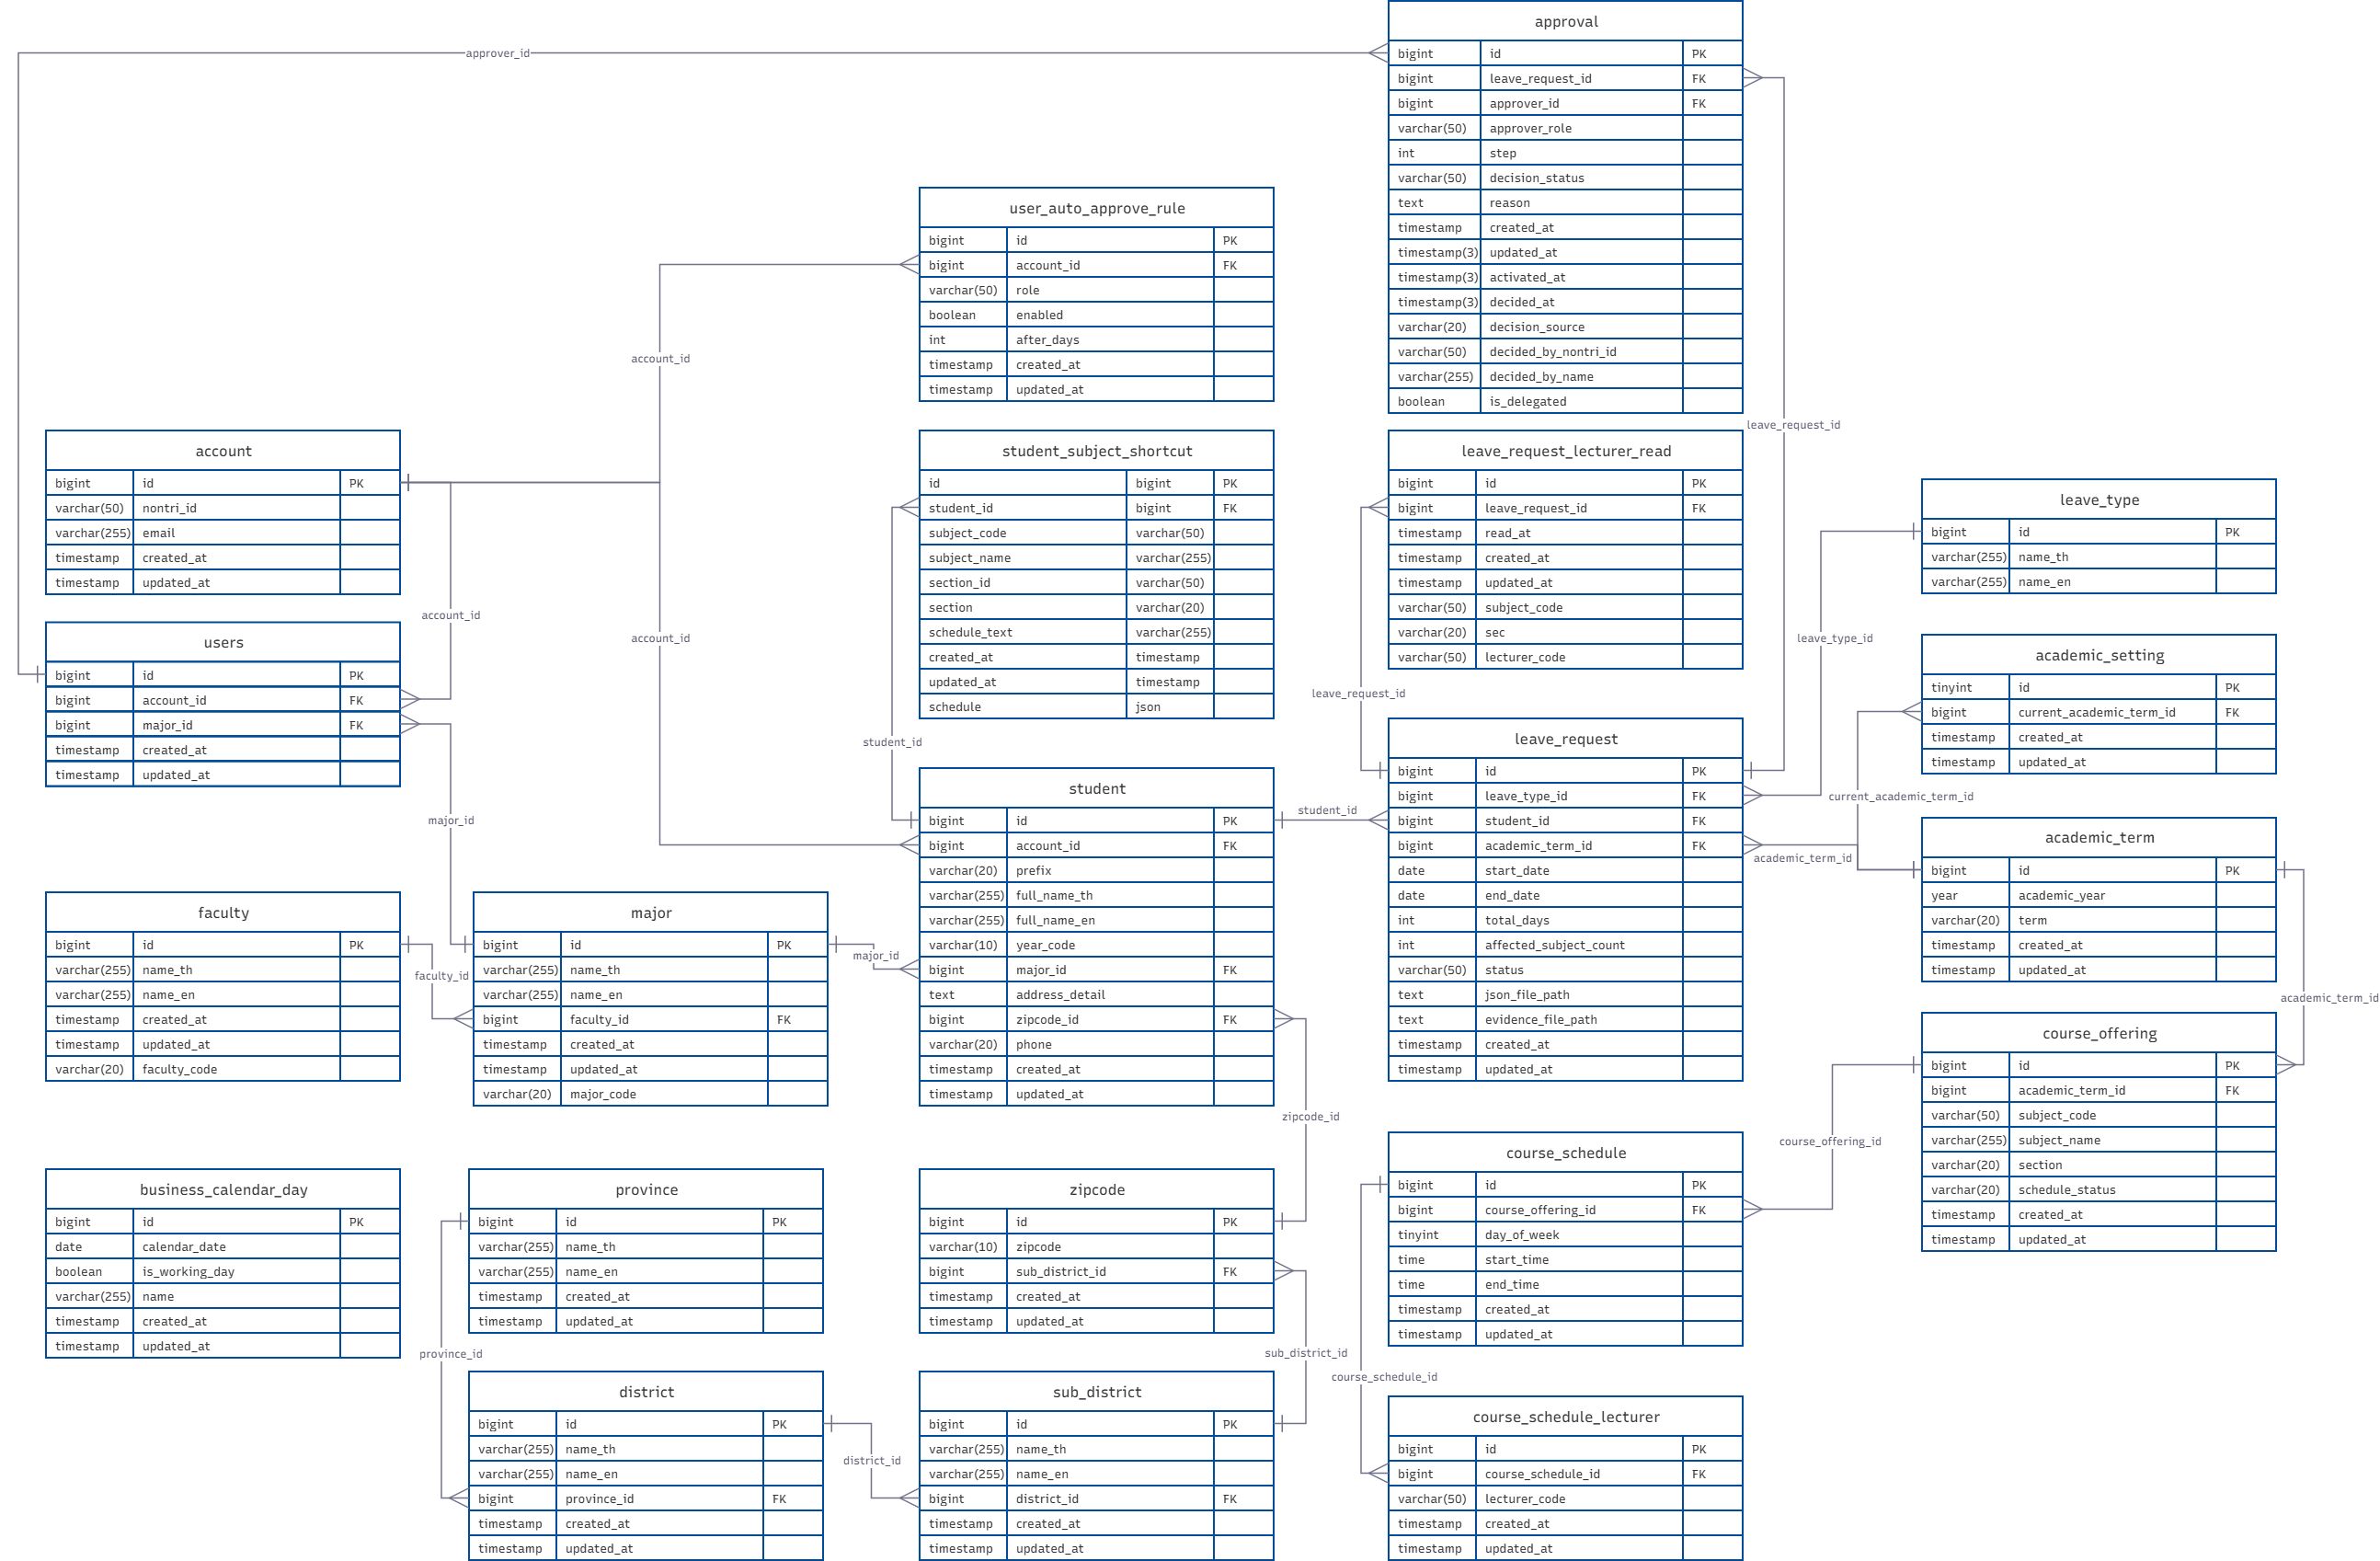
\includegraphics[width=\linewidth,height=145mm,keepaspectratio]{images/leave-schema/DB.png}
\end{center}
\clearpage
\section{ภาพรวมคลังข้อมูล (DW Overview)}
\noindent แผนภาพจากแฟ้ม \texttt{DW-OVERVIEW.png} ที่ผู้จัดทำจัดเตรียม ปรับขนาดตามสัดส่วนให้เต็มพื้นที่หน้าแนวนอน
\begin{center}
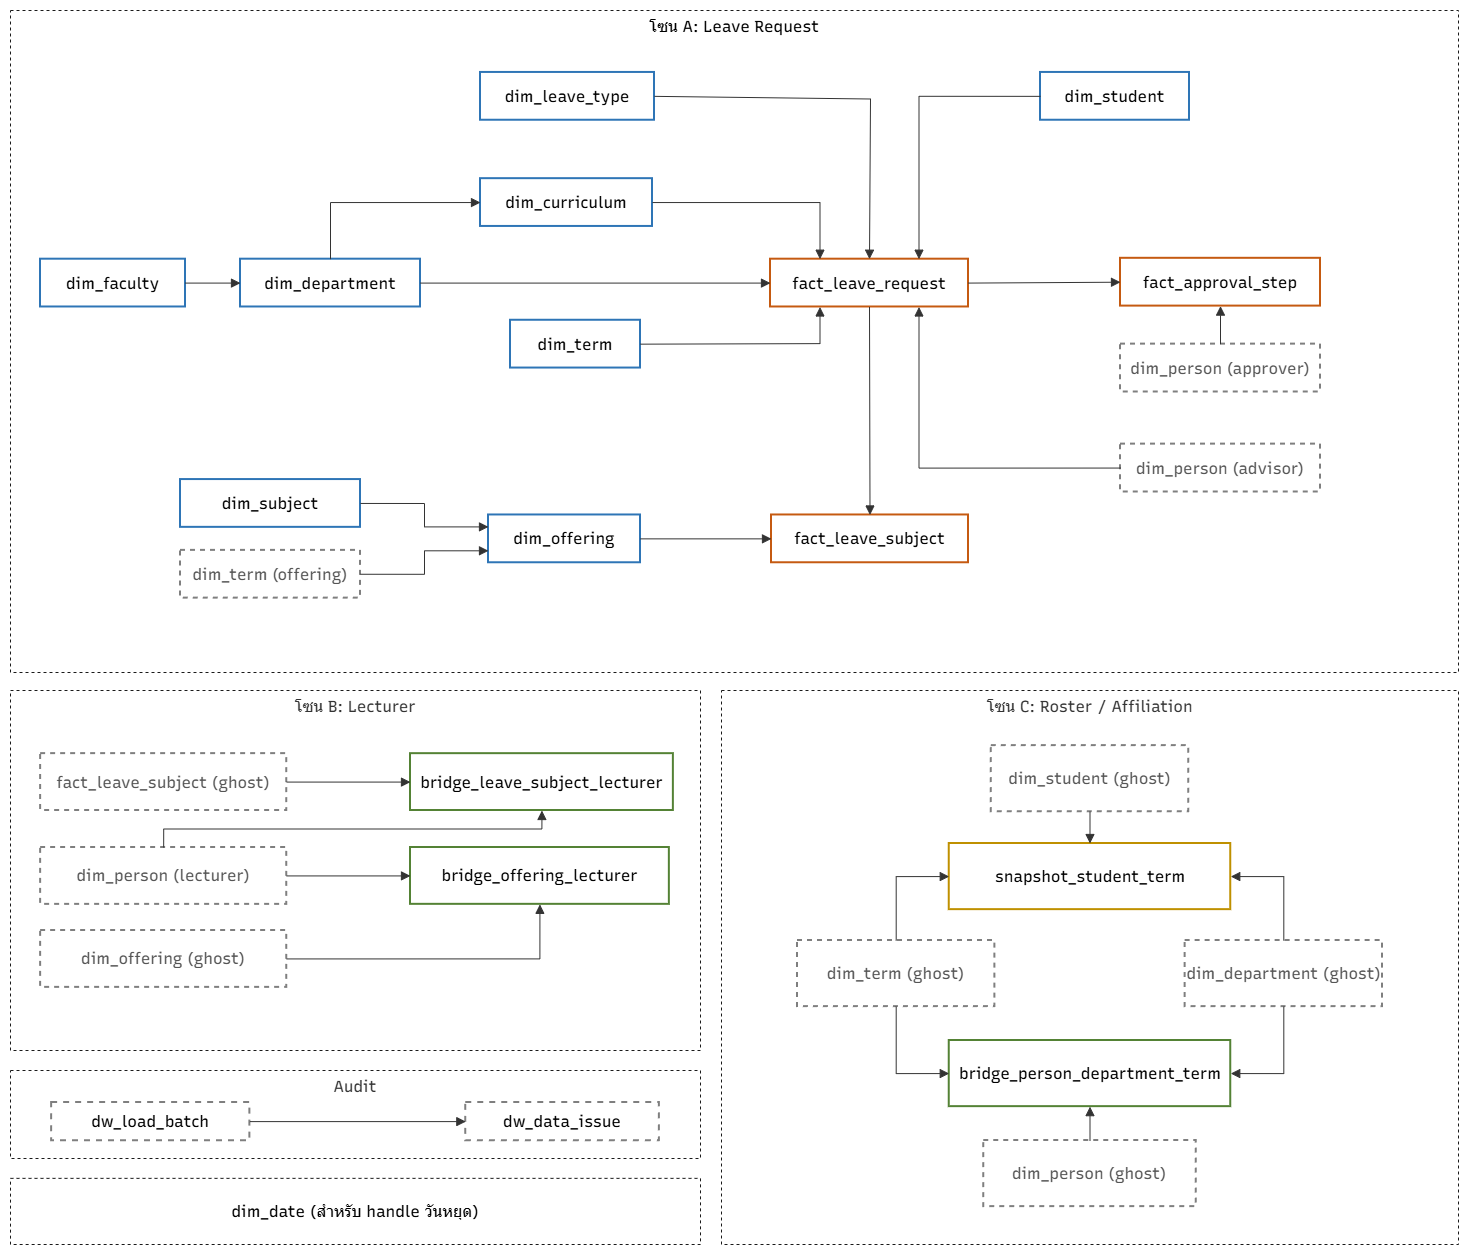
\includegraphics[width=\linewidth,height=145mm,keepaspectratio]{images/leave-schema/DW-OVERVIEW.png}
\end{center}
\clearpage
\section{แผนภาพความสัมพันธ์คลังข้อมูล (DW ERD)}
\noindent แผนภาพจากแฟ้ม \texttt{DW-ERD.png} ที่ผู้จัดทำจัดเตรียม ปรับขนาดตามสัดส่วนให้เต็มพื้นที่หน้าแนวนอน
\begin{center}
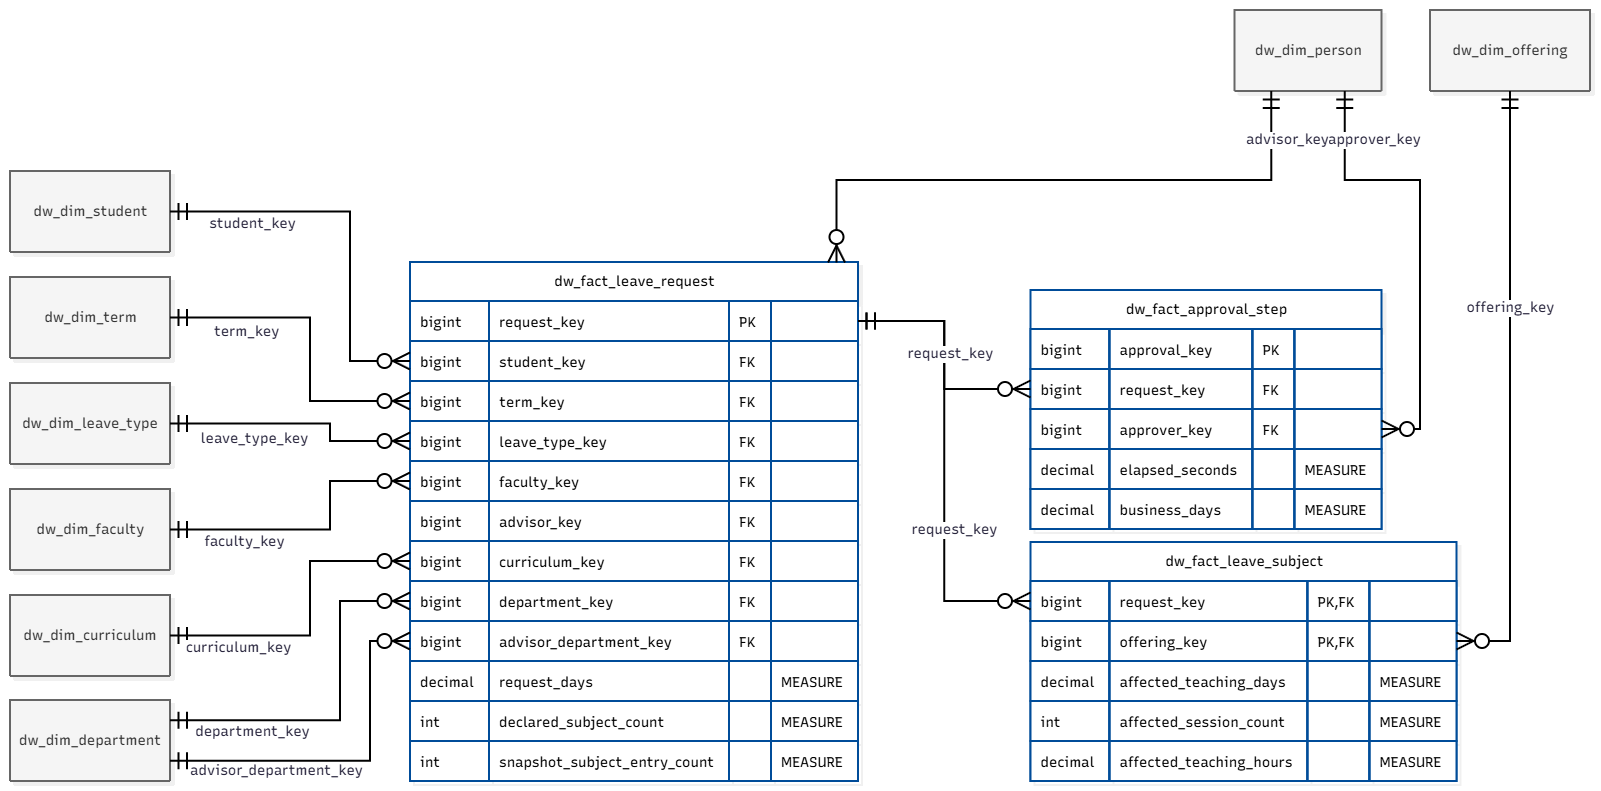
\includegraphics[width=\linewidth,height=145mm,keepaspectratio]{images/leave-schema/DW-ERD.png}
\end{center}
\clearpage
\section{แผนภาพคลังข้อมูลฉบับเต็ม รุ่นที่ 2}
\noindent แผนภาพจากแฟ้ม \texttt{DW-FULL\_VERSION\_2.png} ที่ผู้จัดทำจัดเตรียม ปรับขนาดตามสัดส่วนให้เต็มพื้นที่หน้าแนวนอน
\begin{center}
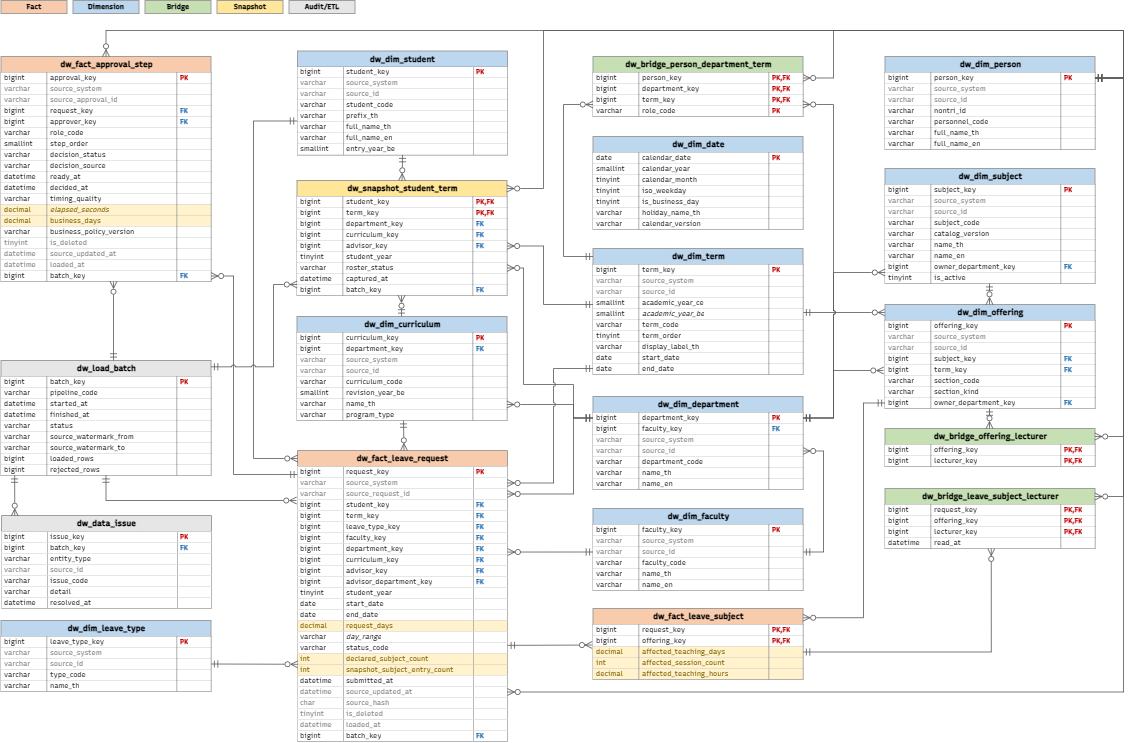
\includegraphics[width=\linewidth,height=145mm,keepaspectratio]{images/leave-schema/DW-FULL_VERSION_2.png}
\end{center}
\clearpage
\section{แผนภาพคอลัมน์ควบคุมคลังข้อมูล}
\noindent แผนภาพจากแฟ้ม \texttt{DW-CONTROL\_COLUMNS.png} ที่ผู้จัดทำจัดเตรียม ปรับขนาดตามสัดส่วนให้เต็มพื้นที่หน้าแนวนอน
\begin{center}
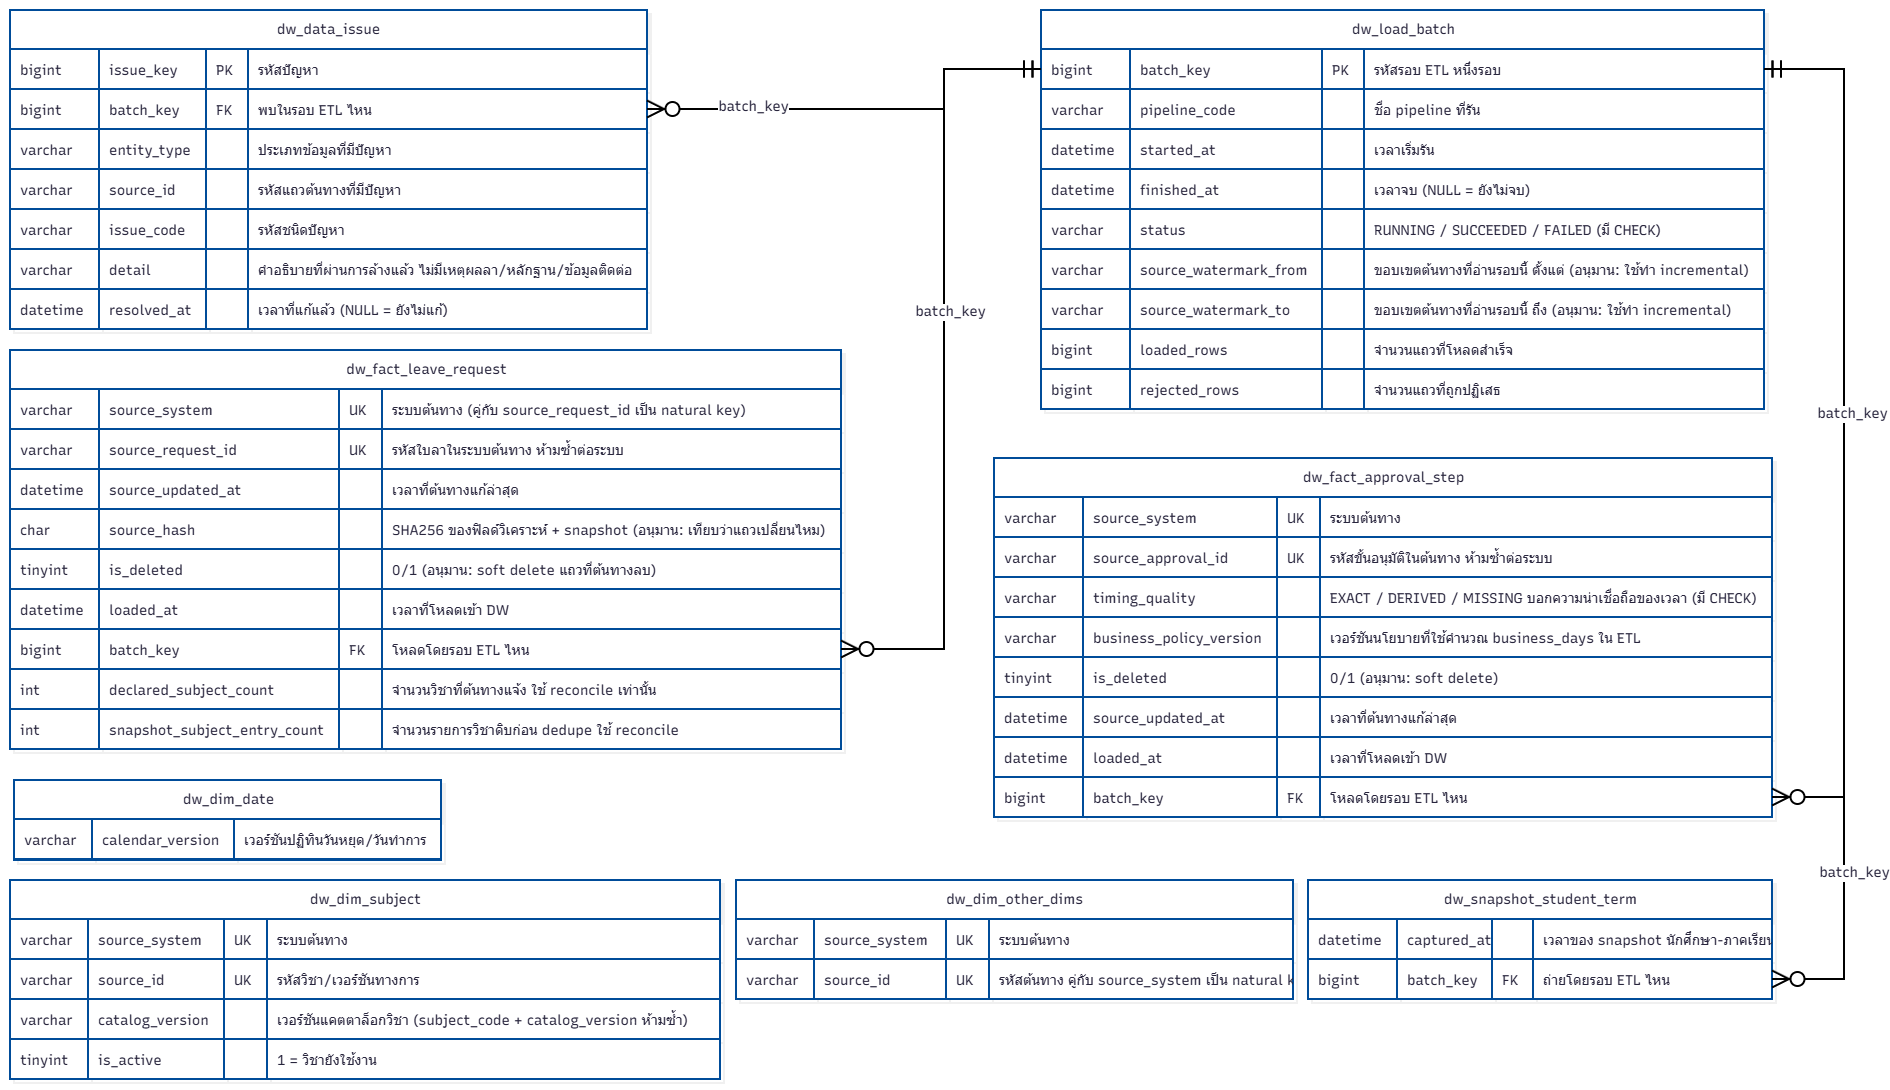
\includegraphics[width=\linewidth,height=145mm,keepaspectratio]{images/leave-schema/DW-CONTROL_COLUMNS.png}
\end{center}
\end{landscape}
